% !TEX root = main.tex
\chapter{Flavour Tagging}
\label{ch:flavourtagging}

To measure interference \CP-violation the production flavour of $B$-mesons under study must be known.
At \lhcb this is inferred using the so-called flavour tagging.
The flavour tagging algorithms (taggers) provide for each candidate both, a decision (tag) $d$ whether it initiallly was a \Bz-meson or a \Bzb-meson and a probability-estimate (mistag) $\eta$ of being wrong with this decision.
They can be divided into two classes: Opposite side (OS) and same side (SS) algorithms.
In this chapter first a general description of the different algorithms available at \lhcb, their performance characteristics and their calibration is given (\cref{sec:taggingalgorithms}).
Following, the tagging strategy for this analysis is outlined in \cref{sec:taggingstrategy} and the calibration of the OS tagging algorithms is summarised (\cref{sec:OScalibration}).
Last the required retraining and the calibration of the SS tagging algorithms presented (\cref{sec:SScalibration}).

\section{Tagging algorithms}
\label{sec:taggingalgorithms}

At \lhcb several tagging algorithms exist to infer the initial $B$ flavour which slightly differ for \Bz and \Bs mesons.
In \cref{fig:taggingalgorithms} a schematic representation of the tagging algorithms for \Bz mesons is shown.
\begin{figure}[tbp]
    \centering
    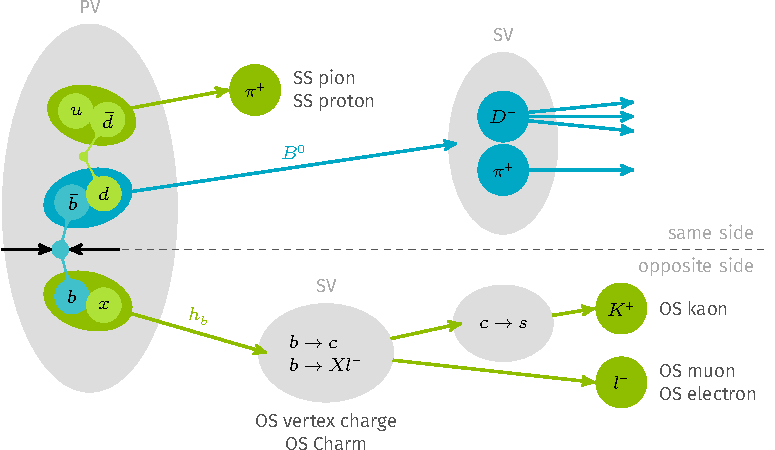
\includegraphics[width=0.8\textwidth]{08FlavourTagging/figs/FTscheme.pdf}
    \caption{Schematic overview of all available \Bz tagging algorithms.}
    \label{fig:taggingalgorithms}
\end{figure}
They can be separated into so-called opposite side (OS) and same side (SS) algorithms.

The OS algorithms exploit the production and decay of the second \bquark-quark which is produced in the proton-proton collision.
By partially reconstructing single decay products as electrons, muons, kaons and \D-mesons associated with the decay of the opposite side \bquark-hadron the initial flavour is inferred.
Furthermore charged tracks which originate from a secondary vertex which is displaced from the \ac{PV} are used to make a decision on the production flavour of the signal $B$-meson.
As the hadronisation and the decay of the OS \bquark-hadron is independent of the signal \B-meson these algorithms can be used for both \Bz and \Bs mesons. Based on \cite{LHCb-PAPER-2011-027, LHCb-PAPER-2015-027} the OS algorithms are shortly described in the following:
\begin{itemize}
	\item The OS muon and OS electron tagger use the charge of muons and electrons from semileptonic $\bquark\!\to Xl^-$ decays to take a decision on the initial $B$-flavour.
	The charged leptons are selected using a simple cut-based selection.
	To suppress contributions from $\bquark\!\to\cquark\!\to l^+$ decays, which would give the wrong tag decision for example the transverse momentum of the muon (electron) is required to be larger than \SI[per-mode=symbol]{1.2}{\GeVc} (\SI[per-mode=symbol]{1.0}{\GeVc}).
	Electrons have additionally to satisfy criteria on electron identification variables such as the ratio $\nicefrac{E}{p}>0.8$.
	Here $E$ denotes the energy deposited in the ECAL and $p$ the electron momentum.
	If more than one muon or electron per event survives the selection, the lepton with highest transverse momentum is chosen to define the flavour of the signal $B$.
	The mistag is estimated with an artificial neural-network, which takes as inputs event properties as the number of \ac{PV}s and tracks in the event, $B$-properties as the transverse momentum, and various geometrical and kinematic properties of the tagging lepton.
	\item The OS kaon tagger explores the charge of kaons produced in the decay chain $\bquark\!\to\cquark\!\to\squark$.
	Very similar to the lepton taggers the tagging kaon is selected using a cut-based selection based on kinematic and PID observables.
	In case multiple kaons per event pass this selection, the kaon with highest transverse momentum is fed into an artificial neural network with similar inputs as for the lepton taggers to calculate the mistag estimate $\eta$.
	\item The OS charm tagger selects \D-mesons produced via $\bquark\!\to\cquark$ decays.
	In case of a charged \D-meson the charge of the meson directly hints at the initial flavour, in case of an uncharged \D-meson the charge of the produced kaon is used to infer the flavour of the signal $B$-meson.
	In contrast to the other single track taggers a \ac{BDT} is used to select the \D-meson and estimate the mistag.
	As the OS charm is the newest development on the OS it was developed to have a small overlap concerning the used tagging particles with the other taggers.
	\item The OS vertex charge tagger is the only algorithm which does not reconstruct single particles, but instead uses the weighted charge of a \ac{SV} associated with the opposite side \bquark-hadron.
	In order to to this, the track pair with the highest probability of originating from the opposite side \bquark-hadron is used to build a vertex.
	Following, particles which are compatible with coming from this two-track vertex but not from the \ac{PV} are added to it.
	Finally all tracks of the final \ac{SV} are weighted with their transverse momentum, \pt, and used to calculate a charge
	\begin{equation}
	Q_{\text{vtx}}=\frac{\sum_{i}p_{\mathrm T}^k(i)Q_i}{\sum_{i}p_{\mathrm T}^k(i)}.
	\end{equation}
	where the parameter $k$ is optimised to maximise the performance of the tagging algorithm.
	Based on this charge then the initial flavour of the signal $B$-meson is determined.
\end{itemize}

The SS algorithms use remnants of the hadronisation of the signal \B-meson to infer the initial flavour.
As the companion quark of the \bquark-quark is different for \Bz and \Bs-mesons, different algorithms must be used to deduce the initial flavour of the signal \B.

In case of a \Bz (\bquarkbar\dquark) a free \dquarkbar-quark is produced which can hadronise to a pion or proton~\cite{Aaij:2016rdg}.
The SS pion and SS proton taggers use the charge of these particles to infer a tag decision.
They were developed on \BdToDpi decays assuming $\Sf=\Sfbar=0$, \ie the decay \BdToDpi is \CP-conserving.
Therefore a potential bias of the analysis cannot be excluded when using these algorithms and they are retrained on $\Bz\!\to\jpsi\Kstarz$.
The basic strategy is similar to the one in Ref.~\cite{Aaij:2016rdg}:
First, tagging particles from the same region of phase space as the signal \B are selected using requirements on PID, kinematic and geometrical observables.
These particles are then all used to train a \ac{BDT}, which further selects the final tagging particle and estimates the mistag.
In case multiple particles per event pass the selection, the SS pion and SS proton taggers do not select the particle with highest transverse momentum, but all particles are used to train the \ac{BDT} and the tagging candidate with the largest \ac{BDT} response is chosen afterwards to infer the initial flavour of the signal \B.

On the other hand the hadronisation of a \Bs (\bquarkbar\squark) leads to a \squarkbar-quark which can hadronise to a kaon~\cite{Aaij:2016psi}.
The SS kaon tagger was developed to identify such kaons and works similar for kaons as the SS pion tagger for pions produced in \Bz events.
Since this analysis covers decays of neutral \Bz mesons and the SS kaon tagger is not used, this algorithm is not discussed here any further.

\subsection{Performance characteristics}

The performance of the flavour tagging algorithms is not perfect.
Of $N$ reconstructed candidates only $N'$ candidates get a tag $d$ and mistag $\eta$ assigned, while $N_{\text{U}}$ are untagged.
The $N'$ candidates can be further divided into $N_{\text{W}}$ candidates which are are wrongly tagged and $N_{\text{R}}$ correctly tagged candidates.
These imperfections can be reflected by a tagging efficiency
\begin{equation}
\varepsilon_{\text{tag}}=\frac{N_{\text{R}}+N_{\text{W}}}{N_{\text{R}}+N_{\text{W}}+N_{\text{R}}+N_{\text{U}}}\label{eq:tageff}
\end{equation}
and a mistag probability
\begin{equation}
\omega=\frac{N_{\text{W}}}{N_{\text{R}}+N_{\text{W}}}.\label{eq:mistag}
\end{equation}
Therefore, in an analysis using flavour tagging to infer the initial \B flavour the number $N_{\Bz}(t)$ ($N_{\Bzb}(t)$) of measured initial \Bz (\Bzb) candidates are
\begin{equation}
\begin{aligned}
N_{\Bz}(t)&=(1-\omega)N_{\Bz}^{\text{true}}(t)+\omega N_{\Bzb}^{\text{true}}(t)\\
N_{\Bzb}(t)&=\omega N_{\Bz}^{\text{true}}(t)+(1-\omega)N_{\Bzb}^{\text{true}}(t).
\end{aligned}
\end{equation}
These quantities need to be transferred further into measurements of \CP-asymmetries such as
\begin{equation}
A_{\CP}(t)=\frac{N_{\Bz}^{\text{true}}(t)-N_{\Bzb}^{\text{true}}(t)}{N_{\Bz}^{\text{true}}(t)+N_{\Bzb}^{\text{true}}(t)}.
\end{equation}
For a measured asymmetry the true numbers of initial \Bz- and \Bzb-mesons need to be replaced with the observed yields what leads to
\begin{equation}
A_{\CP}^{\text{meas}}(t)=\frac{N_{\Bz}(t)-N_{\Bzb}(t)}{N_{\Bz}(t)+N_{\Bzb}(t)}=(1-2\omega)A_{\CP}^{\text{theo}}(t),
\end{equation}
with the dilution $D=1-2\omega$.
However, experimentally not only the dilution affects the measured asymmetry, but also intrinsic asymmetries $I$ like an asymmetric production of \Bz- and \Bzb-mesons might influence a measurement so that the measured asymmetry can be expressed as
\begin{equation}
A_{\CP}^{\text{meas}}(t)=DA_{\CP}(t)+I.
\end{equation}
As the mistag probability is defined in the range $[0, 0.5]$ the dilution can take values between \num{0} and \num{1}.
A large dilution factor is equivalent to a vanishing mistag and hence leads to a larger experimental sensitivity as will be shown below.
To simplify the following discussion the intrinsic asymmetries and dilution are assumed to be time-independent, even if that is not generally valid.
The theoretical asymmetry then can be expressed as
\begin{equation}
A_{\CP}(t)=\frac{1}{D}\left(A_{\CP}^{\text{meas}}(t)-I\right).
\end{equation}
Assuming that all quantities are gaussian distributed the uncertainty on the theoretical asymmetry is given by
\begin{equation}
\begin{aligned}
\sigma_{A_{\CP}}^2&=\left(\frac{\partial A_{\CP}}{\partial N_{\Bz}}\right)^2\sigma_{N_{\Bz}}^2+\left(\frac{\partial A_{\CP}}{\partial N_{\Bzb}}\right)^2\sigma_{N_{\Bzb}}^2+\left(\frac{\partial A_{\CP}}{\partial I}\right)^2\sigma_{I}^2+\left(\frac{\partial A_{\CP}}{\partial D}\right)^2\sigma_{D}^2\\
&=\frac{1}{D^2}\frac{1}{N_{\Bz}(t)+N_{\Bzb}(t)}\left(1-A_{\CP}^{\text{meas}}(t)\right)+\frac{\sigma_{I}^2}{D^2}+\frac{A_{\CP}^2(t)}{D^2}\sigma_{D}^2.
\end{aligned}
\end{equation}
Neglecting the uncertainties on the intrinsic asymmetries and dilution factor and further assuming that the measured asymmetries are small, this expression can be reduced to
\begin{equation}
\sigma_{A_{\CP}}^2=\frac{1}{D^2}\frac{1}{N_{\Bz}(t)+N_{\Bzb}(t)}.
\end{equation}
Here it is useful to identify the number of measured \Bz- and \Bzb-candidates as
\begin{equation}
N_{\Bz}(t)+N_{\Bzb}(t)=\varepsilon(t)N.
\end{equation}
where $\varepsilon$ includes all efficiencies in the trigger, reconstruction, selection or the flavour tagging.
Regarding the flavour tagging this means that the uncertainty on a \CP-asymmetry is given by
\begin{equation}
\sigma_{A_{\CP}}=\frac{1}{\sqrt{\varepsilon_{\text{tag}}D^2N}}=\frac{1}{\sqrt{\varepsilon_{\text{eff}}N}}
\end{equation}
where the effective tagging efficiency $\varepsilon_{\text{eff}}=\varepsilon_{\text{tag}}D^2$ was introduced.
As one can see this efficiency defines the experimental sensitivity of the measurement as it effectively reduces the number of candidates.
It also becomes obvious, that the tagging efficiency introduced in \cref{eq:tageff} and the mistag probability defined in \cref{eq:mistag} are not individually suitable for determining the performance of different tagging algorithms.
Instead the tagging efficiency, which is also denoted as tagging power must be used.

Rather than using an average mistag $\omega$ the mistag estimate $\eta$ of the various tagging algorithms can be used.
To do this, the estimated mistag has to be calibrated with a calibration function $\omega(\eta)$ (more details on the calibration is given in \cref{sec:CombAndCalib}), what gives a per-event tagging power, defined as
\begin{equation}
\varepsilon_{\text{eff}}=\frac{1}{N}\sum_{i=1}^{N}D_i^2=\frac{1}{N}\sum_{i=1}^{N}\left(1-2\omega(\eta_i)\right)^2.
\end{equation}
Here the sum is iterating over all candidates and for untagged candidates the mistag probability is defined to be \num{0.5} ($D_i=0$).

When in an analysis, as in this case, only untagged candidates are considered the effective tagging efficiency reduces to a pseudo tagging power, which is effectively the same as average of the dilution squared in the respective sample:
\begin{equation}
\left<D^2\right>=\frac{1}{N_{\text{R}}+N_{\text{W}}}\sum_{i=1}^{N_{\text{R}}+N_{\text{W}}}\left(1-2\omega(\eta_i)\right)^2.
\end{equation}

\subsection{Combination and calibration of flavour tagging algorithms}
\label{sec:CombAndCalib}

To improve the overall performance of the flavour tagging the individual algorithms are combined to form one single tag decision and mistag for the OS ($d_{\text{OS}}$ and $\eta_{\text{OS}}$) and a tag decision and mistag for the SS ($d_{\text{SS}}$ and $\eta_{\text{SS}}$).
This is done by calculating the combined probability of several taggers, that a \B-meson contains a \bquark-quark as
\begin{equation}
P(\bquark)=\frac{p(\bquark)}{p(\bquark)+p(\bquarkbar)}\hspace{0.5cm}\text{and}\hspace{0.5cm}P(\bquarkbar)=1-P(\bquark).
\end{equation}
The probabilities $p(\bquark)$ and $p(\bquarkbar)$ are defined recursively as
\begin{equation}
p(\bquark)=\prod_{i}\left(\frac{1+d_i}{2}-d_i\left(1-\eta_i\right)\right)
\end{equation}
and
\begin{equation}
p(\bquarkbar)=\prod_{i}\left(\frac{1-d_i}{2}+d_i\left(1-\eta_i\right)\right)
\end{equation}
where $d_i$ ($\eta_i$) are the tag decisions (mistag estimates) of the individual tagging algorithms.
The combined tag decision and mistag are now defined as $d=-1$ and $\eta=1-P(\bquark)$ if $P(\bquark)>P(\bquarkbar)$ and as $d=+1$ and $\eta=P(\bquark)$ if $P(\bquark)<P(\bquarkbar)$.

As mentioned before the output of the flavour tagging algorithms is mostly the result of multivariate classifiers, which are trained on flavour specific \B decays.
This output is then transformed into a mistag estimate $\eta$ and crosschecked on another flavour specific validation sample.
However, the training and validation sample are usually different from the signal decay used in a \CP-violation measurement.
This differences are caused by different trigger and seelction criteria and can influence the distributions which are used by the multivariate classifier to estimate the mistag.
Consequently, the mistag must be calibrated on a dedicated flavour specific decay, which shows at best kinematically similar distributions as the signal sample.
For the OS taggers this is most often done using charged decay modes, as the charge of the final state particles allows to directly infer the production flavour.
Instead, to calibrate the SS taggers a decay mode with the same initial \B flavour is needed, as these taggers highly depend on the hadronisation process.
In this analysis the OS taggers are calibrated using $\Bu\!\to\Dz\pip$, where the bachelor pion allows to infer the initial flavour, while the SS taggers are calibrated using $\Bz\!\to\jpsi\Kstarz$.

So far, for all analyses at \lhcb a linear calibration function of the form
\begin{equation}
\omega(\eta)=\tilde{p}_0+\tilde{p}_1\left(\eta-\left<\eta\right>\right)\label{eq:linCalib}
\end{equation}
where the arithmetic mean $\left<\eta\right>$ of the estimated mistag is used to decorrelate the calibration parameters $p_0$ and $p_1$, was sufficient.
Using this calibration function a perfect calibration would result in $\tilde{p}_0=\left<\eta\right>$ and $\tilde{p}_1=1$.
Yet, the performance of the tagger can depend on the initial \B flavour:
If the interaction rates of charged decay products as kaons used by the OS kaon tagger with the detector material depend on the charge, the mistags will also depend on the flavour of the initial \B meson.
Such asymmetry yields in an additional dilution factor, which needs to be understood and properly described.
This can be achieved by using different calibration functions for \Bz- and \Bzb-mesons.
In the simple linear case these calibration functions are
\begin{equation}
\begin{aligned}
\omega=p_0+p_1+\left(\eta-\left<\eta\right>\right)\\
\overline{\omega}=\overline{p}_0+\overline{p}_1+\left(\eta-\left<\eta\right>\right).
\end{aligned}
\end{equation}
These different calibration parameters are furthermore linked to each other via the average calibration parameters used in \cref{eq:linCalib} and corresponding differences:
\begin{equation}
\tilde{p}_i=\frac{p_i+\overline{p}_i}{2}\hspace{0.5cm}\text{and}\hspace{0.5cm}\Delta p_i=p_i-\overline{p}_i.
\end{equation}

However, this analysis requires more sophisticated calibration models, mainly due to the large number of signal candidates in the \BdToDpi sample.
This makes small effects that were hidden in previous \CP-violation analyses by the statistical ucnertainties significant.
The adopted models are called generalised linear models (GLM)~\cite{GLM} and have the following form:
\begin{equation}
\WorWbar(\eta) = g\left(h(\eta)\right) = g\left( g^{-1} (\eta) + \sum_{i=1}^{N} \left(\tilde{p}_i \kern 0.0em\optbar{\kern -0.0em +} \frac{\Delta p_i}{2}\right) f_i(\eta)\right)\,.
\end{equation}
The functions $f_i$ are the so-called \emph{basis functions}, which for example can be simple poynomials or natural spline functions~\cite{Nsplines}.
To minimise the correlation between the $\tilde{p}_i$ and $\Delta p_i$ parameters the \emph{basis functions} are orthogonalised using the Gram-Schmidt method~\cite{GramSchmidt}.
The function $g$ is referred to as the \emph{link function}, which is usually defined as the inverse cumulative distribution function, to map all input values to the range $[0,1]$, \ie an interval which can be interpreted as a probability.
As the mistag is only defined in the range $[0, 0.5]$ and therefore it is possible, that after applying a calibration function with this \emph{link function} the mistag is larger than \num{0.5}.
In this case an arbitrary decision has to be taken how such candidates are further treated.
Possible options are to either flip the corresponding tag decision $d\to-d$ and adjust the mistag $\omega\to1-\omega$ or to mark the candidate as untagged with a mistag of \num{0.5}.
The latter possibility leads to fit instabilities in the decay-time fit when the calibration parameters are not fixed, but allowed to float or constrained by means of a Gaussian function.
This is due to the fact, that for a floating or constrained calibration the ratio of tagged and untagged candidates varies during the minimisation and the changes to the likeihood are not continous.
On the other hand, a flip of the tagdesicion may yield in a bias of the \CP-parameters as shown in \cref{sec:decTimeFitVal}.
Therefore, the modified logistic function
\begin{equation}
g(h)=\frac{1}{2\left(1+e^h\right)}
\end{equation}
is used as \emph{link function}, which maps all input values into the range $[0, 0.5]$ and hence assures that all calibrated mistags are well defined.

To not rely on possible binning effects on the estimated msitag $\eta$ or the mistag probabilitz $\omega$, the calibration functions are determined using an unbinned maximum-likelihood method, the so-called binomial regression~\cite{BinRegression}.

\section{Flavour tagging strategy}
\label{sec:taggingstrategy}

In this analysis the combination of all available OS taggers is used, while for the SS both taggers designed to tag the initial flavour of \Bz-mesons are combined into one single tag decision and mistag.
The OS taggers were all developed and trained on a datasample of $\Bu\!\to\jpsi\Kp$ decays, except for the OS charm tagger, whose BDT was trained on a mixed sample of simulated $\Bu\!\to\jpsi\Kp$, $\Bz\!\to\jpsi\Kstarz$ and $\Bs\!\to\jpsi\phi$ decays.
As the OS taggers are independent of the initial signal \B they can be used in this default version.
As control channel the decay $\Bu\!\to\Dz\pip$ is used.
As mentioned before, the SS pion and the SS proton taggers were deveolped and trained on a datasample of \BdToDpi decays, assuming no \CP-violation.
The use of these algorithms could therefor bias the measurement of \Sf and \Sfbar and hence both taggers are retrained (more details given in \cref{sec:retrainSSpion} and \cref{sec:retrainSSproton}).

To include the flavour tagging in the decay rates given in \crefrange{eq:DecRateB2Dmpip}{eq:DecRateBb2Dppim} the expressions for the \CP-parameters \Sf and \Cf need to be extended to
\begin{equation}
\begin{aligned}
\Sf\to\left(\Delta^--\Delta^+\right)\Sf\\
\Cf\to\left(\Delta^--\Delta^+\right)\Cf.
\end{aligned}
\end{equation}
Similar equations hold also for \Sfbar and \Cfbar.
The coefficients $\Delta^\pm$ contain the calibration functions and tagging efficiencies $\varepsilon_{\text{tag}}^{\text{OS}}$ and $\varepsilon_{\text{tag}}^{\text{SS}}$.
They are defined as
\begin{align}
\Delta^\pm&=\frac{1}{2}\varepsilon_{\text{\tiny tag}}^{\text{\tiny OS}}\left[1-\varepsilon_{\text{\tiny tag}}^{\text{\tiny SS}}+d^{\text{\tiny OS}}\left(1-\varepsilon_{\text{\tiny tag}}^{\text{\tiny SS}}-2\omega(\eta^{\text{\tiny OS}})\left(1+\varepsilon_{\text{\tiny tag}}^{\text{\tiny SS}}\right)\right)\right]\nonumber\\
&\pm\frac{1}{2}\varepsilon_{\text{\tiny tag}}^{\text{\tiny OS}}\left[1-\varepsilon_{\text{\tiny tag}}^{\text{\tiny SS}}+d^{\text{\tiny OS}}\left(1-\varepsilon_{\text{\tiny tag}}^{\text{\tiny SS}}-2\overline{\omega}(\eta^{\text{\tiny OS}})\left(1+\varepsilon_{\text{\tiny tag}}^{\text{\tiny SS}}\right)\right)\right]
\end{align}
for candidates which are only tagged by the OS tagger combination.
To obtain the expression for candidates only tagged by the SS taggers, all superscripts need to be exchanged with $\text{OS}\leftrightarrow\text{SS}$.
For candidates which are tagged by both, the OS tagger combination and the SS taggers the coefficients can be written as
\begin{align}
\Delta^\pm&=\frac{1}{4}\varepsilon_{\text{\tiny tag}}^{\text{\tiny OS}}\varepsilon_{\text{\tiny tag}}^{\text{\tiny SS}}\left[1+\hspace{-3mm}\sum_{j=\text{\tiny OS, SS}}\hspace{-2mm}d_j\left(1-2\omega(\eta_j)\right)+d^{\text{\tiny OS}}d^{\text{\tiny SS}}\left(1-2\omega(\eta_j)+2\omega(\eta^{\text{\tiny OS}})\omega(\eta^{\text{\tiny SS}})\right)\right]\nonumber\\
&\pm\frac{1}{4}\varepsilon_{\text{\tiny tag}}^{\text{\tiny OS}}\varepsilon_{\text{\tiny tag}}^{\text{\tiny SS}}\left[1+\hspace{-3mm}\sum_{j=\text{\tiny OS, SS}}\hspace{-2mm}d_j\left(1-2\overline{\omega}(\eta_j)\right)+d^{\text{\tiny OS}}d^{\text{\tiny SS}}\left(1-2\overline{\omega}(\eta_j)+2\overline{\omega}(\eta^{\text{\tiny OS}})\overline{\omega}(\eta^{\text{\tiny SS}})\right)\right].
\end{align}

The flavour specific control samples ($\Bu\!\to\Dz\pip$ for the OS, $\Bz\!\to\jpsi\Kstarz$ for the SS) are used to determine the functional form of the calibration function $\omega(\eta)$.
Unlike other flavour tagged analyses at \lhcb the calibration parameter are determined directly in the decay-time fit as floating nuisance parameter of the likelihood function in \BdToDpi.
This is possible because the parameters \Cf and \Cfbar are fixed to \num{1} and \num{-1} as the ratio $r$ (see \cref{eq:ratioDpi}) is expected too small to allow a significant measurement of both parameters.
As a result, the cosine term allows to determine the calibration parameters independently of the sine term.
A qualitative explaination is given in \cref{fig:FTstrategy}.
A more quantitative validation was done by a collaboratoron pseudoexperiments:
Generating pseudoexperiments and floating the parameters \Cf and \Cfbar in the fit showed a non-negligible bias for the parameters \Sf and \Sfbar, while fixing the coefficients \Cf and \Cfbar in the fit showed unbiased results on all fitted parameters.
Finally it should be noted here, that possible deviations from the assumption of $\Cf=-\Cfbar=1$ are taken into account in the systematic uncertainties.
\begin{figure}[tbp]
    \centering
    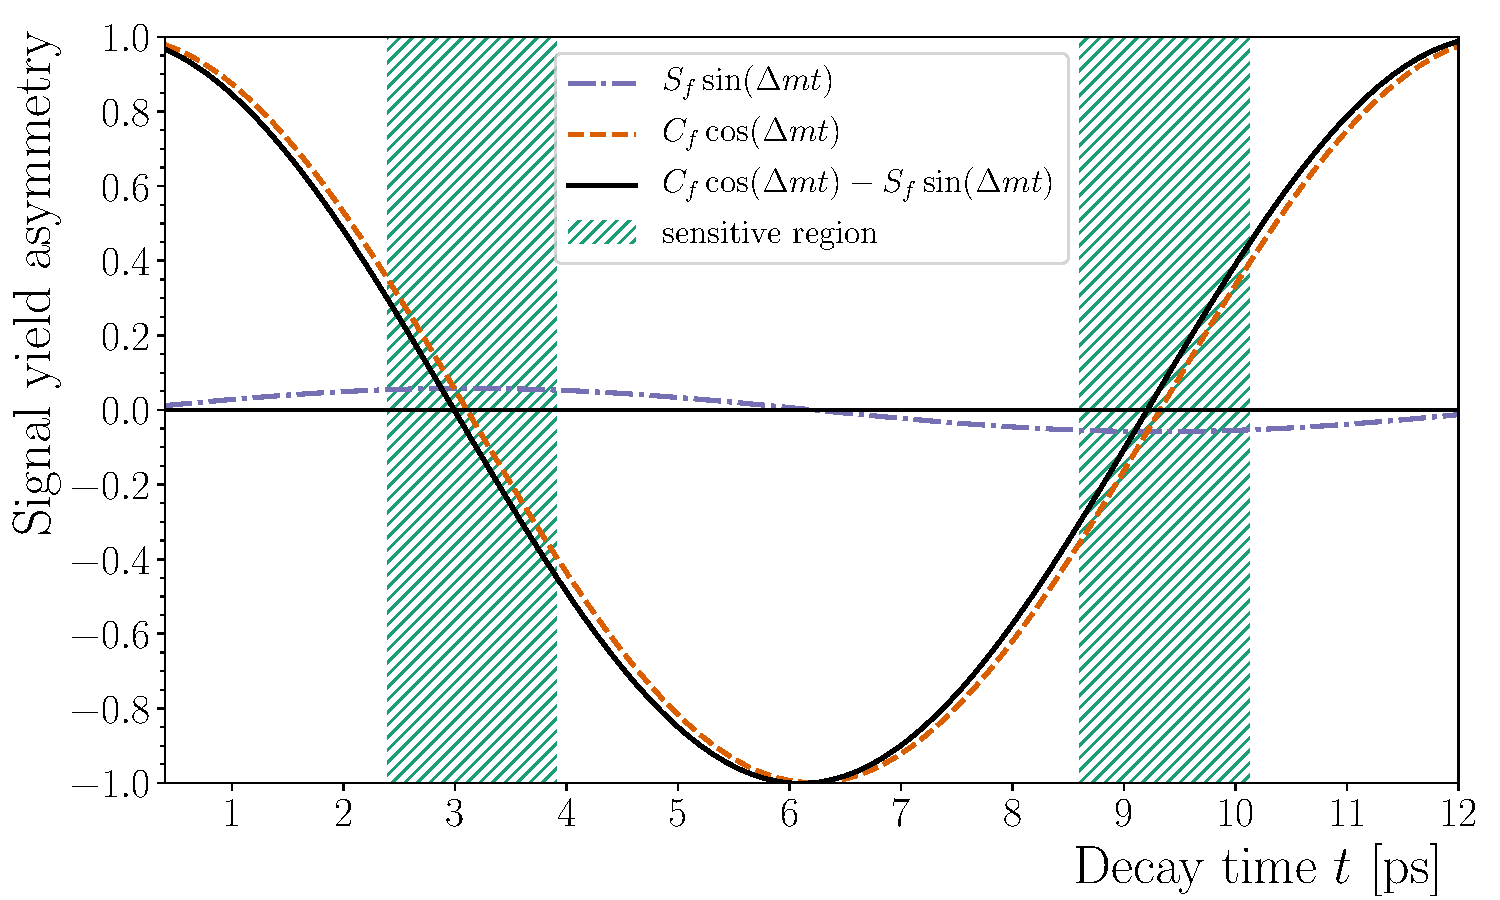
\includegraphics[width=0.48\textwidth]{08FlavourTagging/figs/oscillation_f.pdf}
    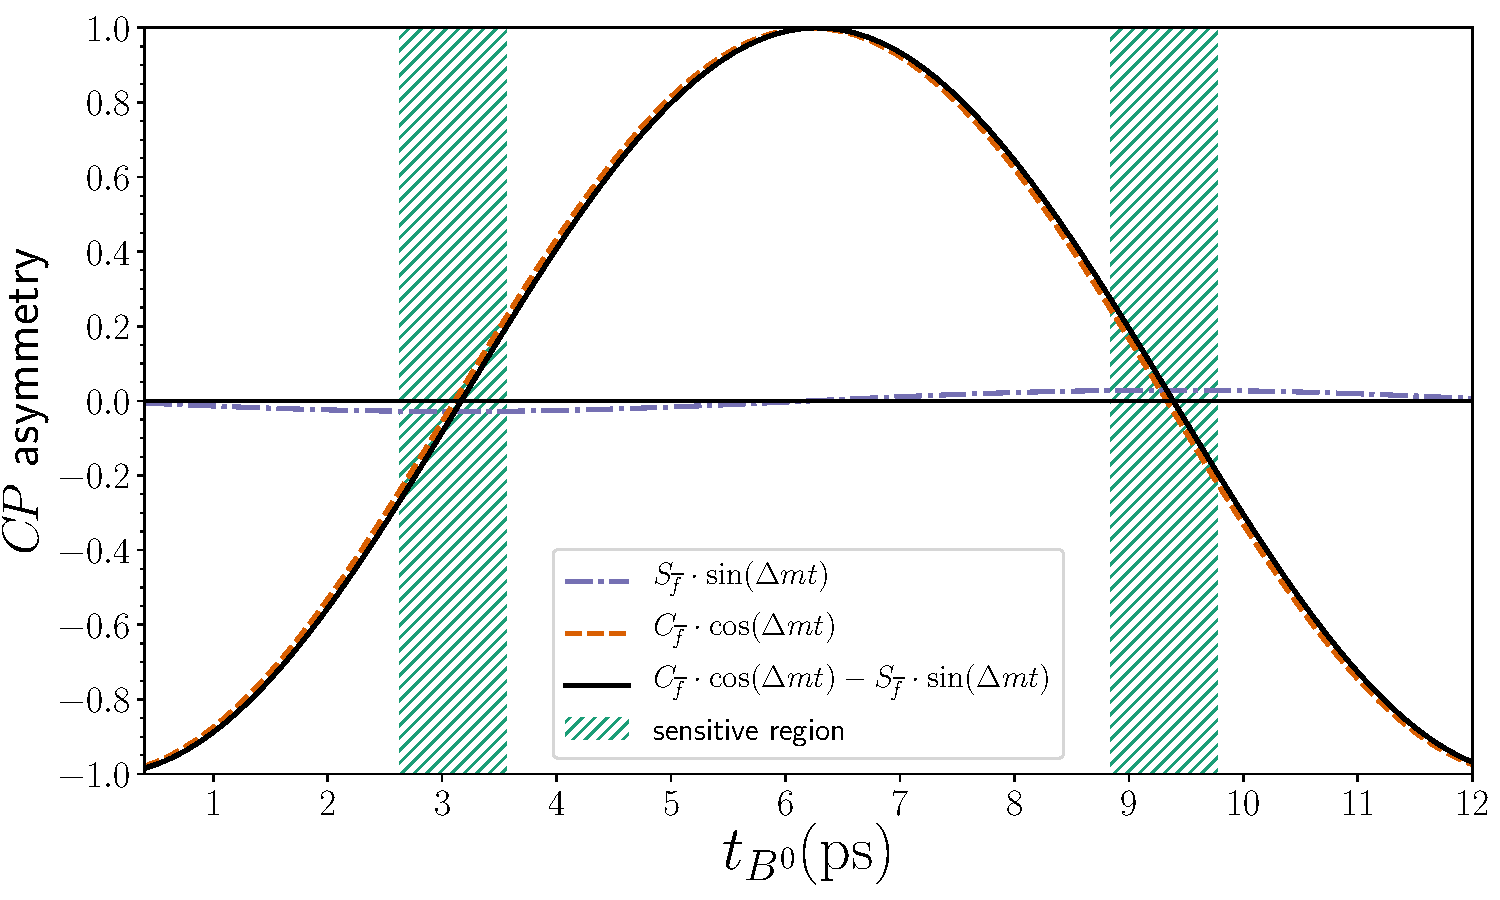
\includegraphics[width=0.48\textwidth]{08FlavourTagging/figs/oscillation_fbar.pdf}
    \caption{Time-dependent asymmetries for \Bzb versus \Bz for the \Dm\pip (left) and \Dp\pim (right) final states.
    The values for the \CP parameters are taken from simulation and no experimental dilutions are included.
    Since the deviation of the sum of both trigonometric functions from a single cosine function is very small due to the tiny values of \Sf and \Sfbar, the maximum sensitivity is achieved in the regions of the zero-points, \ie where the amplitude of $\cos(\dm t)$ and $\sin(\dm t)$ are of similar size.
    These regions are denoted as \enquote{sensitive regions} in both plots.
    In the \enquote{non-sensitive regions}, where the cosine-function is completely dominating, additional diluting effects due to the tagging calibration can be determined.}
    \label{fig:FTstrategy}
\end{figure}

As all calibration parameters are directly determined in the signal sample no assumptions for the portability of the calibration from a control channel is needed.
However, the additional degrees of freedom in the final decay-time fit lead to an increased statistical uncertainty on the \CP-parameters \Sf and \Sfbar.
This is compensated by the fact, that the systematic uncertainty for the portability of the calibration, which is often the largest systematic uncertainty for flavour tagged analyses at \lhcb, is needed.
Such systematic uncertainty would be accounting for kinematic differences between the control sample and the signal sample leading to different flavour tagging calibrations.
To check the portability simulated events of both, the control sample and the signal sample are used.
When checking the portability of the calibrations from $\Bu\!\to\Dz\pip$ and $\Bz\!\to\jpsi\Kstarz$ to \BdToDpi a bias on \Sf and \Sfbar of roughly the size of their statistical uncertainty arises.
This bias can be reduced, when floating the calibration parameters (more details on this are given in \cref{sec:decTimeFitVal}).
Furthermore, the precision of the calibration parameters for the SS tagger combination obtained in the decay-time fit to \BdToDpi is much smaller compared to the precision on the control channel, while for the OS tagger combination the uncertainty on the signal sample increases only slightly compared to the uncertainty obtained on the control sample.

Therefore, the studies presented in the following sections do not aim, to obtain the calibration parameters.
Instead, on the one hand, they are used to determine the functional form of the calibration function, which is used in the decay-time fit described in \cref{sec:ExtractCPobs}.
On the other hand, the obtained parameter values of the calibration function can be used as reference values for the decay-time fit, as even if they are not expected to agree perfectly, both parameter sets should be in the same interval.

\section{Opposite side tagging calibration}
\label{sec:OScalibration}


\section{Same side tagging calibration}
\label{sec:SScalibration}

\subsection[head={Selection and mass fit of $\Bz\!\to\jpsi\Kstarz$ candidates},tocentry={Selection and mass fit of $\Bz\!\to\jpsi\Kstarz$ candidates}]{Selection and mass fit of $\symbfsf{\Bz\!\to\jpsi\Kstarz}$ candidates}


\subsection{Retraining of the SS pion tagger}
\label{sec:retrainSSpion}


\subsection{Retraining of the SS proton tagger}
\label{sec:retrainSSproton}

\subsection{Calibration portability}
